\documentclass[aspectratio=169,11pt]{beamer}

\usetheme{Madrid}
\usecolortheme{seahorse}
\setbeamertemplate{navigation symbols}{}
\setbeamertemplate{caption}[numbered]

\usepackage[utf8]{inputenc}
\usepackage[T1]{fontenc}
\usepackage[spanish,es-nodecimaldot]{babel}
\usepackage{amsmath,amssymb,amsfonts}
\usepackage{booktabs}
\usepackage{array}
\usepackage{graphicx}
\usepackage{tikz}
\usepackage{xcolor}

\graphicspath{{outputs_sbm_sw/}}

\definecolor{deepblue}{HTML}{243B53}
\definecolor{accentred}{HTML}{D1495B}
\definecolor{accentgreen}{HTML}{4C956C}
\definecolor{accentorange}{HTML}{F28C61}
\definecolor{accentpurple}{HTML}{7C6AAC}

\setbeamercolor{title}{fg=deepblue}
\setbeamercolor{frametitle}{fg=deepblue}
\setbeamercolor{block title}{bg=deepblue!12,fg=deepblue}
\setbeamercolor{block body}{bg=deepblue!4,fg=black}
\setbeamercolor{alerted text}{fg=accentred}

\newcommand{\Gmini}{G_{\mathrm{mini}}}
\newcommand{\Omhat}{\hat\Omega}
\newcommand{\what}{\hat\omega}

\title[DC-SBM Star Wars II]{Inferencia estadística de comunidades con DC-SBM}
\subtitle{Caso de estudio: red de personajes de \emph{Star Wars II: Attack of the Clones}}
\author{LDS1121 - Redes complejas}
\date{}

\begin{document}

% ------------------------------------------------------------
\begin{frame}
  \titlepage
\end{frame}

% ------------------------------------------------------------
\begin{frame}{Objetivo de la presentación}
\begin{block}{Pregunta principal}
¿La red de personajes se organiza como comunidades densas, como roles narrativos que conectan subtramas, o como una mezcla?
\end{block}

\vspace{0.3cm}

\begin{itemize}
    \item Usamos el archivo \texttt{data/dataverse/gexf/774.gexf}.
    \item La película es \emph{Star Wars II: Attack of the Clones}.
    \item Ajustamos un modelo de bloques estocásticos corregido por grado.
    \item Interpretamos las comunidades con $M=(m_{rs})$ y $\Omhat=(\what_{rs})$.
\end{itemize}

\vspace{0.25cm}
\begin{alertblock}{Idea central}
El DC-SBM no solo encuentra grupos densos: también encuentra \textbf{roles} y \textbf{puentes narrativos}.
\end{alertblock}
\end{frame}

% ------------------------------------------------------------
\begin{frame}{Datos usados}
\begin{columns}[T,totalwidth=\textwidth]
\begin{column}{0.50\textwidth}
\begin{block}{Lectura del archivo}
\small
\begin{align*}
\texttt{PROJECT\_ROOT} &= \texttt{find\_project\_root()}\\
\texttt{folder} &= \texttt{PROJECT\_ROOT/data/dataverse/gexf}\\
\texttt{movie\_id} &= 774\\
\texttt{fp} &= \texttt{folder}/\texttt{774.gexf}
\end{align*}
\end{block}

\begin{itemize}
    \item Grafo no dirigido.
    \item Nodos: personajes.
    \item Aristas: coaparición o interacción.
    \item Etiquetas: nombres de personajes.
\end{itemize}
\end{column}

\begin{column}{0.47\textwidth}
\begin{block}{Red completa y minired}
\centering
\begin{tabular}{lrrrr}
\toprule
Red & Nodos & Aristas & Densidad & Grado prom.\\
\midrule
$G$ & 47 & 148 & 0.137 & 6.30\\
$\Gmini$ & 34 & 128 & 0.228 & 7.53\\
\bottomrule
\end{tabular}
\end{block}

\vspace{0.2cm}
\small
La minired conserva personajes con grado al menos $3$:
\[
V_{\mathrm{mini}}=\{i\in V:\; k_i\ge 3\}.
\]
\end{column}
\end{columns}
\end{frame}

% ------------------------------------------------------------
\begin{frame}{Por qué usar una minired}
\begin{columns}[T,totalwidth=\textwidth]
\begin{column}{0.48\textwidth}
\begin{block}{Red completa}
\begin{itemize}
    \item Conserva todos los personajes.
    \item Incluye apariciones periféricas.
    \item Permite ver el contexto narrativo completo.
\end{itemize}
\end{block}
\end{column}

\begin{column}{0.48\textwidth}
\begin{block}{Minired}
\begin{itemize}
    \item Elimina personajes con grado $1$ o $2$.
    \item Destaca el núcleo de interacción.
    \item Ayuda a ver si la estructura central se mantiene.
\end{itemize}
\end{block}
\end{column}
\end{columns}

\vspace{0.35cm}
\begin{alertblock}{Interpretación}
La minired no reemplaza a la red completa. Funciona como prueba de sensibilidad: si una historia aparece en ambas, es más robusta.
\end{alertblock}
\end{frame}

% ------------------------------------------------------------
\begin{frame}{Personajes más conectados}
\centering
\begin{tabular}{lr@{\qquad}lr}
\toprule
Personaje & Grado & Personaje & Grado\\
\midrule
PADMÉ & 30 & YODA & 14\\
OBI-WAN & 29 & MACE WINDU & 13\\
ANAKIN & 24 & JAR JAR & 11\\
PALPATINE & 11 & MAS AMEDDA & 10\\
SENATOR ASK AAK & 10 & BAIL ORGANA & 9\\
COUNT DOOKU & 9 & AMIDALA & 6\\
CAPTAIN TYPHO & 6 & JANGO FETT & 6\\
NUTE GUNRAY & 6 & POGGLE & 6\\
\bottomrule
\end{tabular}

\vspace{0.4cm}

\begin{block}{Lectura narrativa}
Padmé, Obi-Wan y Anakin dominan por grado. Por eso necesitamos corregir por grado: de otro modo, la partición podría confundir centralidad individual con comunidad.
\end{block}
\end{frame}

% ------------------------------------------------------------
\begin{frame}{Modelo: DC-SBM}
\begin{block}{Asignación latente}
Cada personaje $i$ pertenece a un grupo
\[
g_i\in\{1,\ldots,q\}.
\]
\end{block}

\begin{block}{Modelo de aristas}
La intensidad esperada de arista entre $i$ y $j$ es proporcional a
\[
\omega_{g_i g_j}\frac{c_i c_j}{2m}.
\]
\end{block}

\begin{itemize}
    \item $c_i$: grado esperado o propensión individual del personaje $i$.
    \item $\omega_{rs}$: intensidad de interacción entre grupos $r$ y $s$.
    \item $2m=\sum_i k_i$: volumen total de grado.
\end{itemize}
\end{frame}

% ------------------------------------------------------------
\begin{frame}{Notación de bloques}
Para una partición fija $g$:
\[
\kappa_r=\sum_i\delta_{g_i r}c_i,
\qquad
m_{rs}=\sum_{ij}\delta_{g_i r}\delta_{g_j s}A_{ij}.
\]

\vspace{0.25cm}

\begin{columns}[T,totalwidth=\textwidth]
\begin{column}{0.48\textwidth}
\begin{block}{$\kappa_r$}
Volumen de grado del grupo $r$.
\[
\kappa_r=\text{suma de propensiones del grupo }r.
\]
\end{block}
\end{column}
\begin{column}{0.48\textwidth}
\begin{block}{$m_{rs}$}
Masa observada de aristas entre $r$ y $s$.
\[
M=(m_{rs}) \text{ resume la red por bloques.}
\]
\end{block}
\end{column}
\end{columns}
\end{frame}

% ------------------------------------------------------------
\begin{frame}{Estimadores de máxima verosimilitud}
Al maximizar respecto a los parámetros continuos:
\[
\hat c_i=k_i,
\qquad
\what_{rs}=\frac{2m\,m_{rs}}{\kappa_r\kappa_s}.
\]

\vspace{0.3cm}

\begin{alertblock}{Por qué esto importa}
\[
\what_{rs}
\neq
\text{``número de aristas''}.
\]
Mide cuántas aristas hay entre $r$ y $s$ \textbf{relativas a lo esperado por grado}.
\end{alertblock}

\begin{itemize}
    \item Si $\what_{rr}$ es alta: grupo internamente denso.
    \item Si $\what_{rs}$ es alta con $r\neq s$: relación entre roles o subtramas.
\end{itemize}
\end{frame}

% ------------------------------------------------------------
\begin{frame}{Log-verosimilitud perfilada}
Sustituyendo $\hat c_i$ y $\what_{rs}$:
\[
L(g)=
\frac{1}{2}\sum_{r,s}
m_{rs}\log\left(\frac{m_{rs}}{\kappa_r\kappa_s}\right)
+\text{constantes}.
\]

\vspace{0.35cm}

\begin{block}{Problema computacional}
\[
\hat g_q=\arg\max_{g:V\to\{1,\ldots,q\}}L(g).
\]
\end{block}

\begin{itemize}
    \item Se fija $q$.
    \item Se buscan etiquetas $g_i$ que aumenten $L(g)$.
    \item Se repite con varios arranques aleatorios.
\end{itemize}
\end{frame}

% ------------------------------------------------------------
\begin{frame}{Cómo se hizo en la notebook}
\begin{enumerate}
    \item Leer el grafo GEXF y relabelar nodos con nombres de personajes.
    \item Construir la red completa $G$ y la minired $\Gmini$.
    \item Para cada $q$, ajustar DC-SBM con múltiples arranques.
    \item Calcular $M$, $\Omhat$, $\kappa_r$ y modularidad diagnóstica.
    \item Escoger $q$ con un criterio penalizado tipo BIC.
    \item Dibujar red, matrices y vistas focales.
\end{enumerate}

\vspace{0.25cm}
\begin{block}{Criterio penalizado}
\[
\operatorname{BIC}_{\mathrm{like}}(q)
=-2\hat L_q+p_q\log(2m),
\qquad
p_q\approx \frac{q(q+1)}2-q.
\]
\end{block}
\end{frame}

% ------------------------------------------------------------
\begin{frame}{Selección de $q$: red completa}
\centering
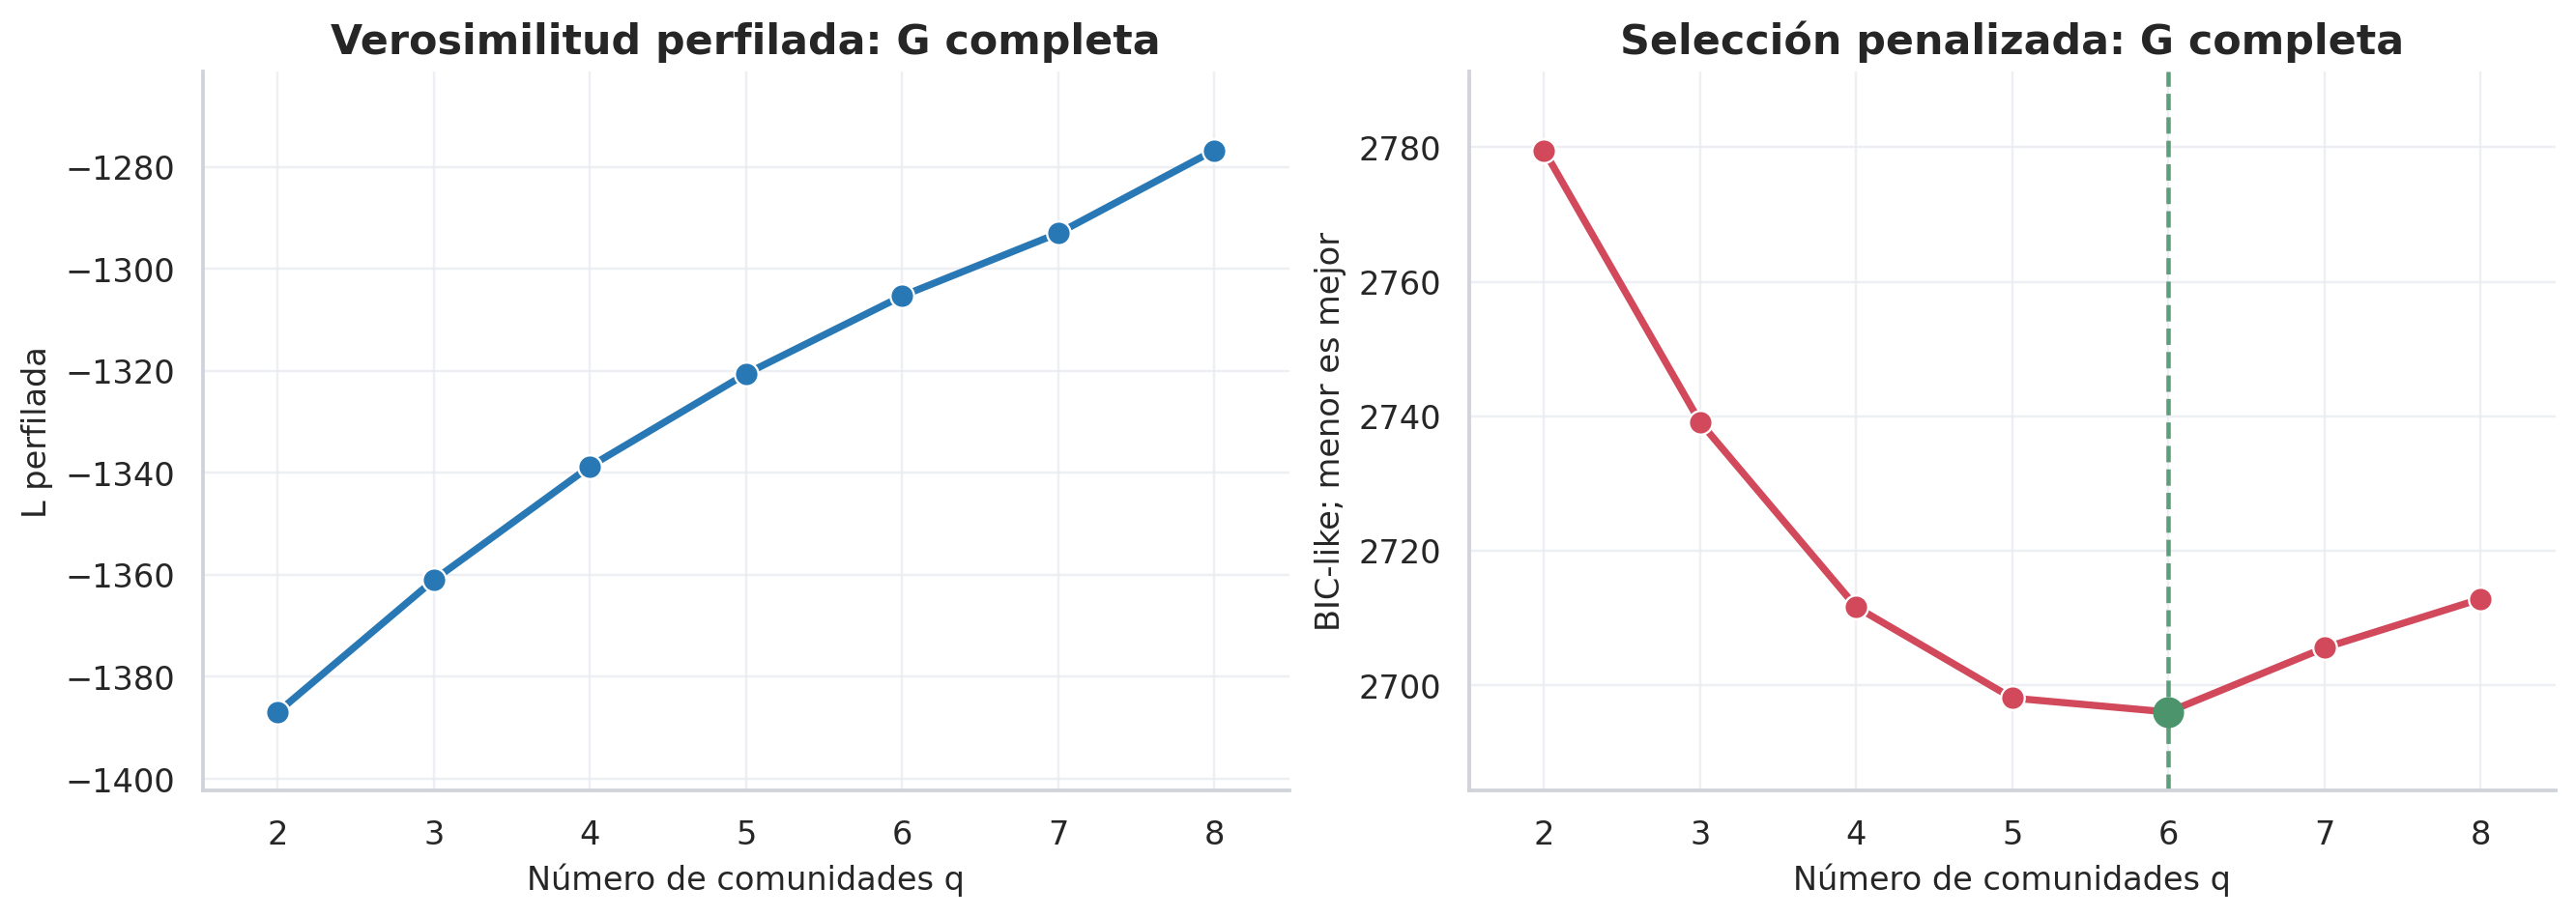
\includegraphics[width=0.82\textwidth]{barrido_q_G_completa.png}

\vspace{0.15cm}
\begin{block}{Resultado}
Para la red completa, el BIC-like selecciona
\[
q=6.
\]
\end{block}
\end{frame}

% ------------------------------------------------------------
\begin{frame}{Selección de $q$: minired}
\centering

\includegraphics[width=0.82\textwidth]{barrido_q_G_mini.png}

\vspace{0.15cm}
\begin{block}{Resultado}
Para la minired, el BIC-like selecciona
\[
q=5.
\]
\end{block}
\end{frame}

% ------------------------------------------------------------
\begin{frame}{Tabla del barrido de $q$}
\centering
\scriptsize
\begin{tabular}{llrrr}
\toprule
Red & $q$ & $L$ perfilada & BIC-like & Modularidad\\
\midrule
$G$ & 2 & -1386.927 & 2779.544 & 0.248\\
$G$ & 3 & -1361.020 & 2739.110 & 0.125\\
$G$ & 4 & -1338.741 & 2711.623 & 0.183\\
$G$ & 5 & -1320.584 & 2698.073 & 0.212\\
$G$ & 6 & -1305.318 & \alert{2695.992} & 0.146\\
$G$ & 7 & -1293.018 & 2705.534 & 0.117\\
$G$ & 8 & -1276.739 & 2712.808 & 0.145\\
\midrule
$\Gmini$ & 2 & -1228.973 & 2463.491 & 0.251\\
$\Gmini$ & 3 & -1206.781 & 2430.197 & 0.114\\
$\Gmini$ & 4 & -1187.248 & 2407.767 & 0.175\\
$\Gmini$ & 5 & -1172.257 & \alert{2399.965} & 0.140\\
$\Gmini$ & 6 & -1159.504 & 2402.186 & 0.165\\
$\Gmini$ & 7 & -1149.048 & 2414.545 & 0.167\\
\bottomrule
\end{tabular}

\vspace{0.25cm}
\begin{alertblock}{Interpretación}
La modularidad no es máxima en esos puntos, porque el SBM no busca solo comunidades cerradas: también detecta roles y cruces entre subtramas.
\end{alertblock}
\end{frame}

% ------------------------------------------------------------
\section{Red completa}

\begin{frame}{Red completa: comunidades estimadas}
\scriptsize
\centering
\begin{tabular}{clrrp{7.2cm}}
\toprule
Grupo & Lectura & Nodos & Int. & Miembros principales\\
\midrule
1 & Padmé y conectores periféricos & 6 & 0 & DARTH SIDIOUS, ELAN, PADMÉ, SHMI, WATTO, ZAM WESSEL\\
2 & Tatooine/Naboo/separatistas periféricos & 13 & 12 & BERU, CLIEGG, NUTE GUNRAY, OWEN, POGGLE, QUEEN JAMILLIA, THREEPIO\\
3 & Obi-Wan como puente & 2 & 0 & DOOKU, OBI-WAN\\
4 & Eje Anakin/Dooku & 2 & 1 & ANAKIN, COUNT DOOKU\\
5 & Kamino/Jango & 9 & 8 & BOBA FETT, JANGO, JANGO FETT, LAMA SU, TAUN WE\\
6 & Senado/Jedi/República & 15 & 41 & AMIDALA, BAIL ORGANA, JAR JAR, MACE WINDU, PALPATINE, YODA\\
\bottomrule
\end{tabular}

\vspace{0.25cm}
\begin{block}{Lectura}
La partición no separa solo por ``facciones''. También aísla personajes puente y subtramas muy concentradas.
\end{block}
\end{frame}

% ------------------------------------------------------------
\begin{frame}{Red completa: volúmenes y aristas}
\centering
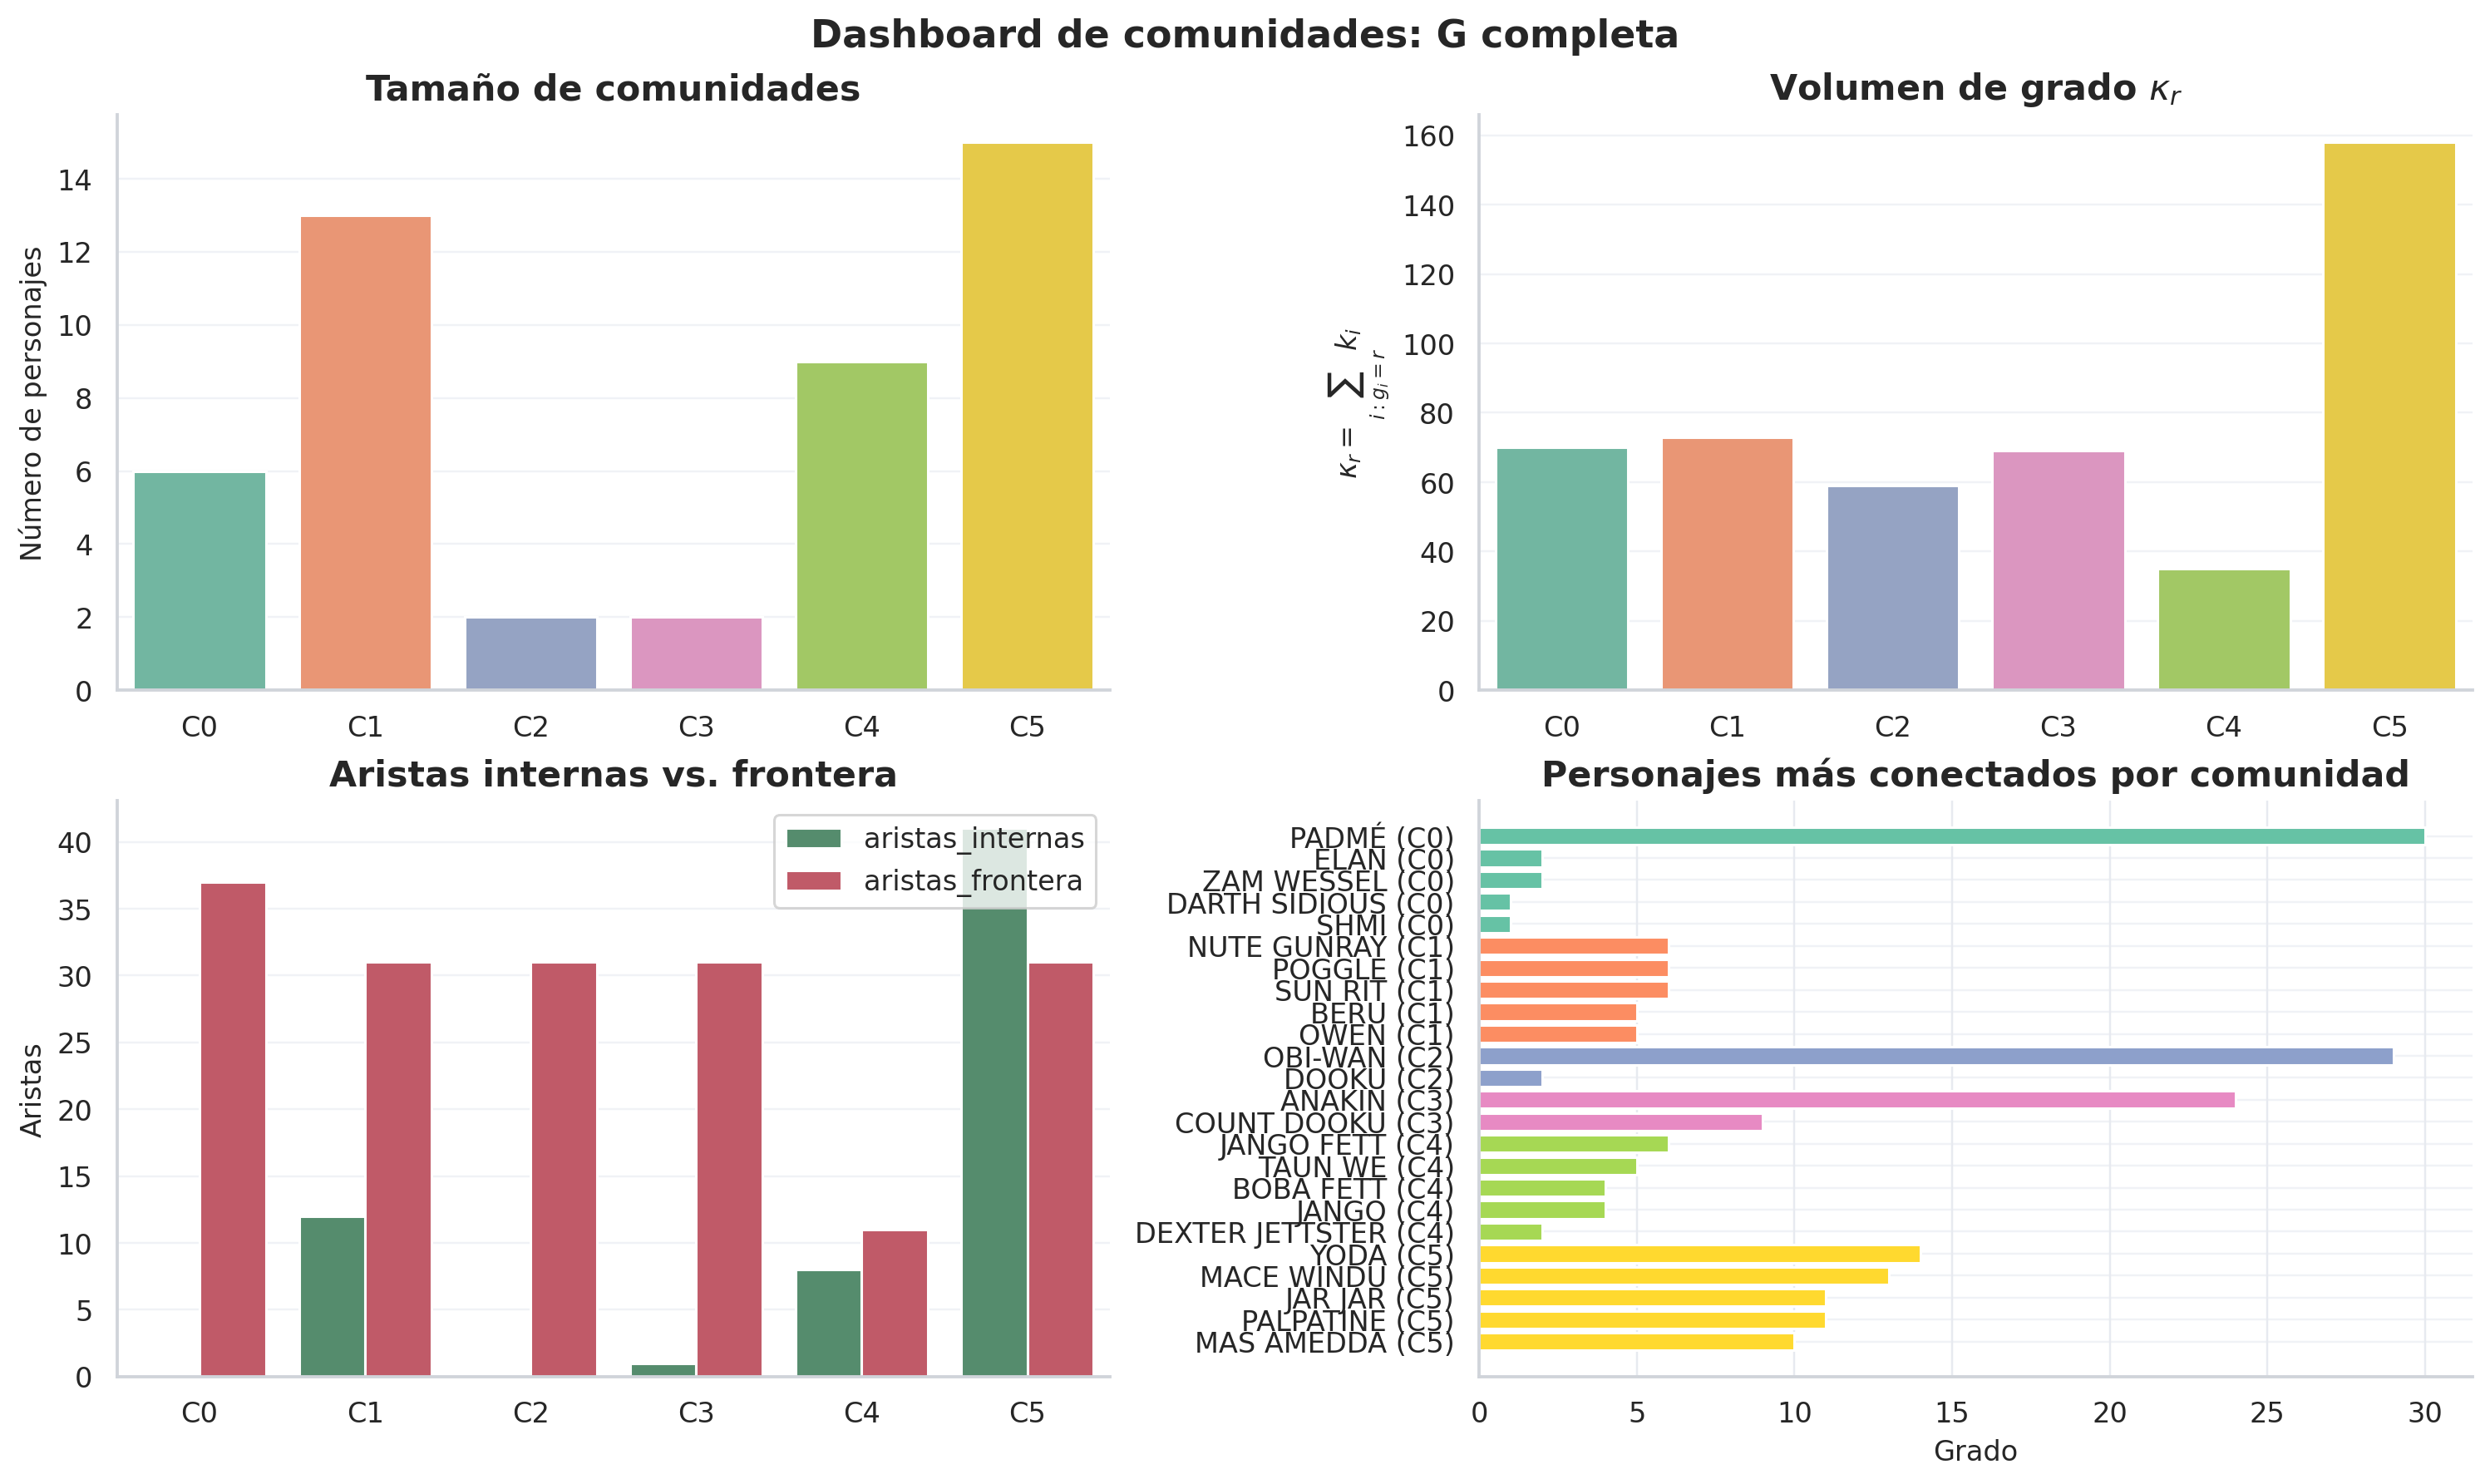
\includegraphics[height=0.58\textheight]{dashboard_comunidades_G_completa.png}

\vspace{0.05cm}
\begin{block}{Interpretación}
\small
El grupo 6 tiene gran volumen de grado y muchas aristas internas. El grupo 5 es pequeño, pero muy concentrado: Kamino/Jango aparece como subtrama compacta.
\end{block}
\end{frame}

% ------------------------------------------------------------
\begin{frame}{Red completa: matriz $M$}
\scriptsize
\[
M=
\begin{pmatrix}
0&19&7&25&1&18\\
19&34&3&17&0&0\\
7&3&0&14&16&19\\
25&17&14&2&0&11\\
1&0&16&0&18&0\\
18&0&19&11&0&110
\end{pmatrix}
\]

\begin{block}{Qué dice $M$}
\begin{itemize}
    \item $m_{66}=110$: mucha masa interna en Senado/Jedi/República.
    \item $m_{55}=18$: masa interna del bloque Kamino/Jango.
    \item $m_{35}=16$: conexión Obi-Wan/Kamino-Jango.
    \item $m_{14}=25$: conexión Padmé--Anakin/Dooku.
\end{itemize}
\end{block}
\end{frame}

% ------------------------------------------------------------
\begin{frame}{Red completa: matriz $\Omhat$}
\scriptsize
\[
\Omhat=
\begin{pmatrix}
0&1.725&0.786&2.402&0.189&0.755\\
1.725&2.960&0.323&1.566&0&0\\
0.786&0.323&0&1.596&3.595&0.946\\
2.402&1.566&1.596&0.195&0&0.468\\
0.189&0&3.595&0&6.818&0\\
0.755&0&0.946&0.468&0&2.045
\end{pmatrix}
\]

\begin{alertblock}{Lectura clave}
El valor más alto es $\what_{55}=6.818$: Kamino/Jango es una subtrama muy cerrada después de corregir por grado. El cruce más fuerte fuera de la diagonal es $\what_{35}=3.595$: Obi-Wan conecta con Kamino/Jango más de lo esperado.
\end{alertblock}
\end{frame}

% ------------------------------------------------------------
\begin{frame}{Radiografía de bloques: red completa}
\centering
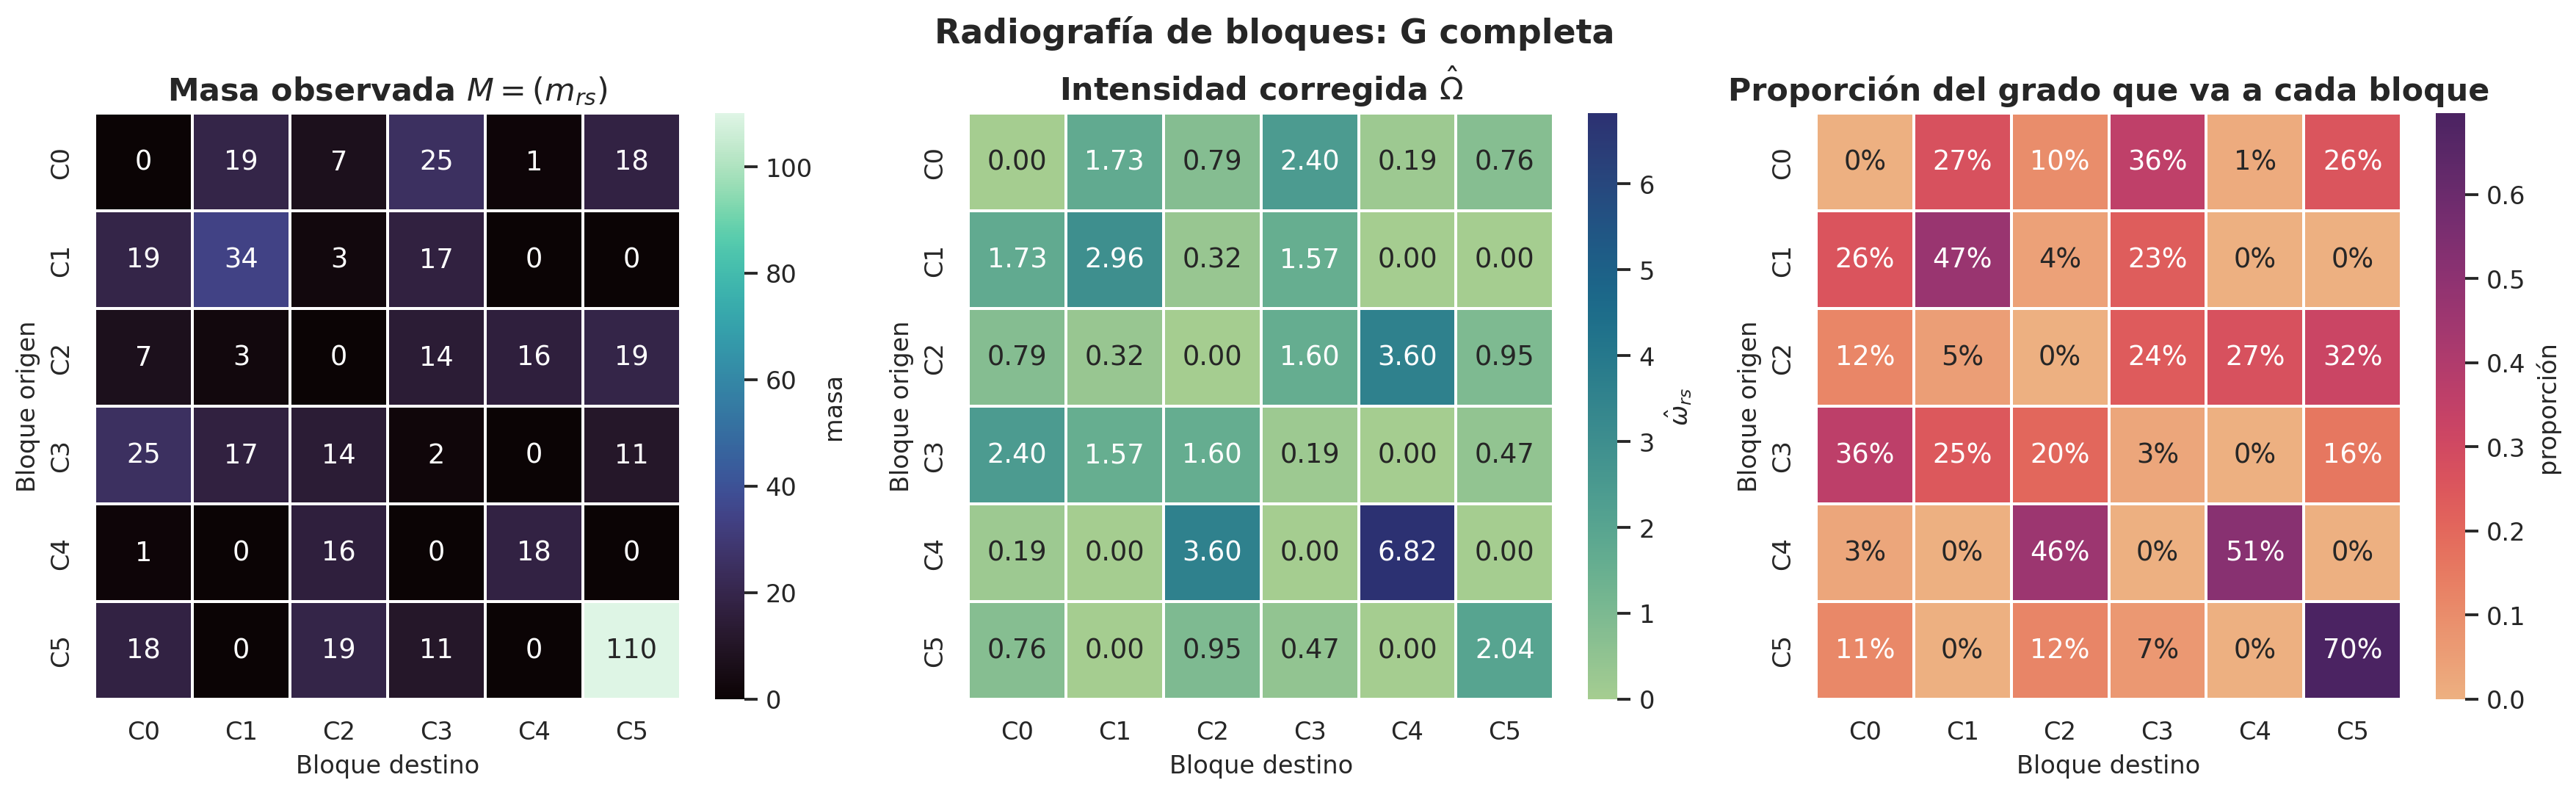
\includegraphics[width=0.96\textwidth]{radiografia_bloques_G_completa.png}
\end{frame}

% ------------------------------------------------------------
\begin{frame}{Interpretación de la radiografía}
\begin{columns}[T,totalwidth=\textwidth]
\begin{column}{0.48\textwidth}
\begin{block}{Diagonales fuertes}
\begin{itemize}
    \item Grupo 5: Kamino/Jango.
    \item Grupo 2: Tatooine/Naboo periférico.
    \item Grupo 6: Senado/Jedi/República.
\end{itemize}
\end{block}
\end{column}
\begin{column}{0.48\textwidth}
\begin{block}{Cruces fuertes}
\begin{itemize}
    \item Grupo 3--5: Obi-Wan con Kamino/Jango.
    \item Grupo 1--4: Padmé con Anakin/Dooku.
    \item Grupo 1--2: conectores hacia bloque familiar/periférico.
\end{itemize}
\end{block}
\end{column}
\end{columns}

\vspace{0.25cm}
\begin{alertblock}{Conclusión parcial}
La película no se comporta como una red con comunidades aisladas. Tiene subtramas densas, pero también personajes que sirven de bisagra.
\end{alertblock}
\end{frame}

% ------------------------------------------------------------
\begin{frame}{Cruce dominante: Obi-Wan y Kamino/Jango}
\centering
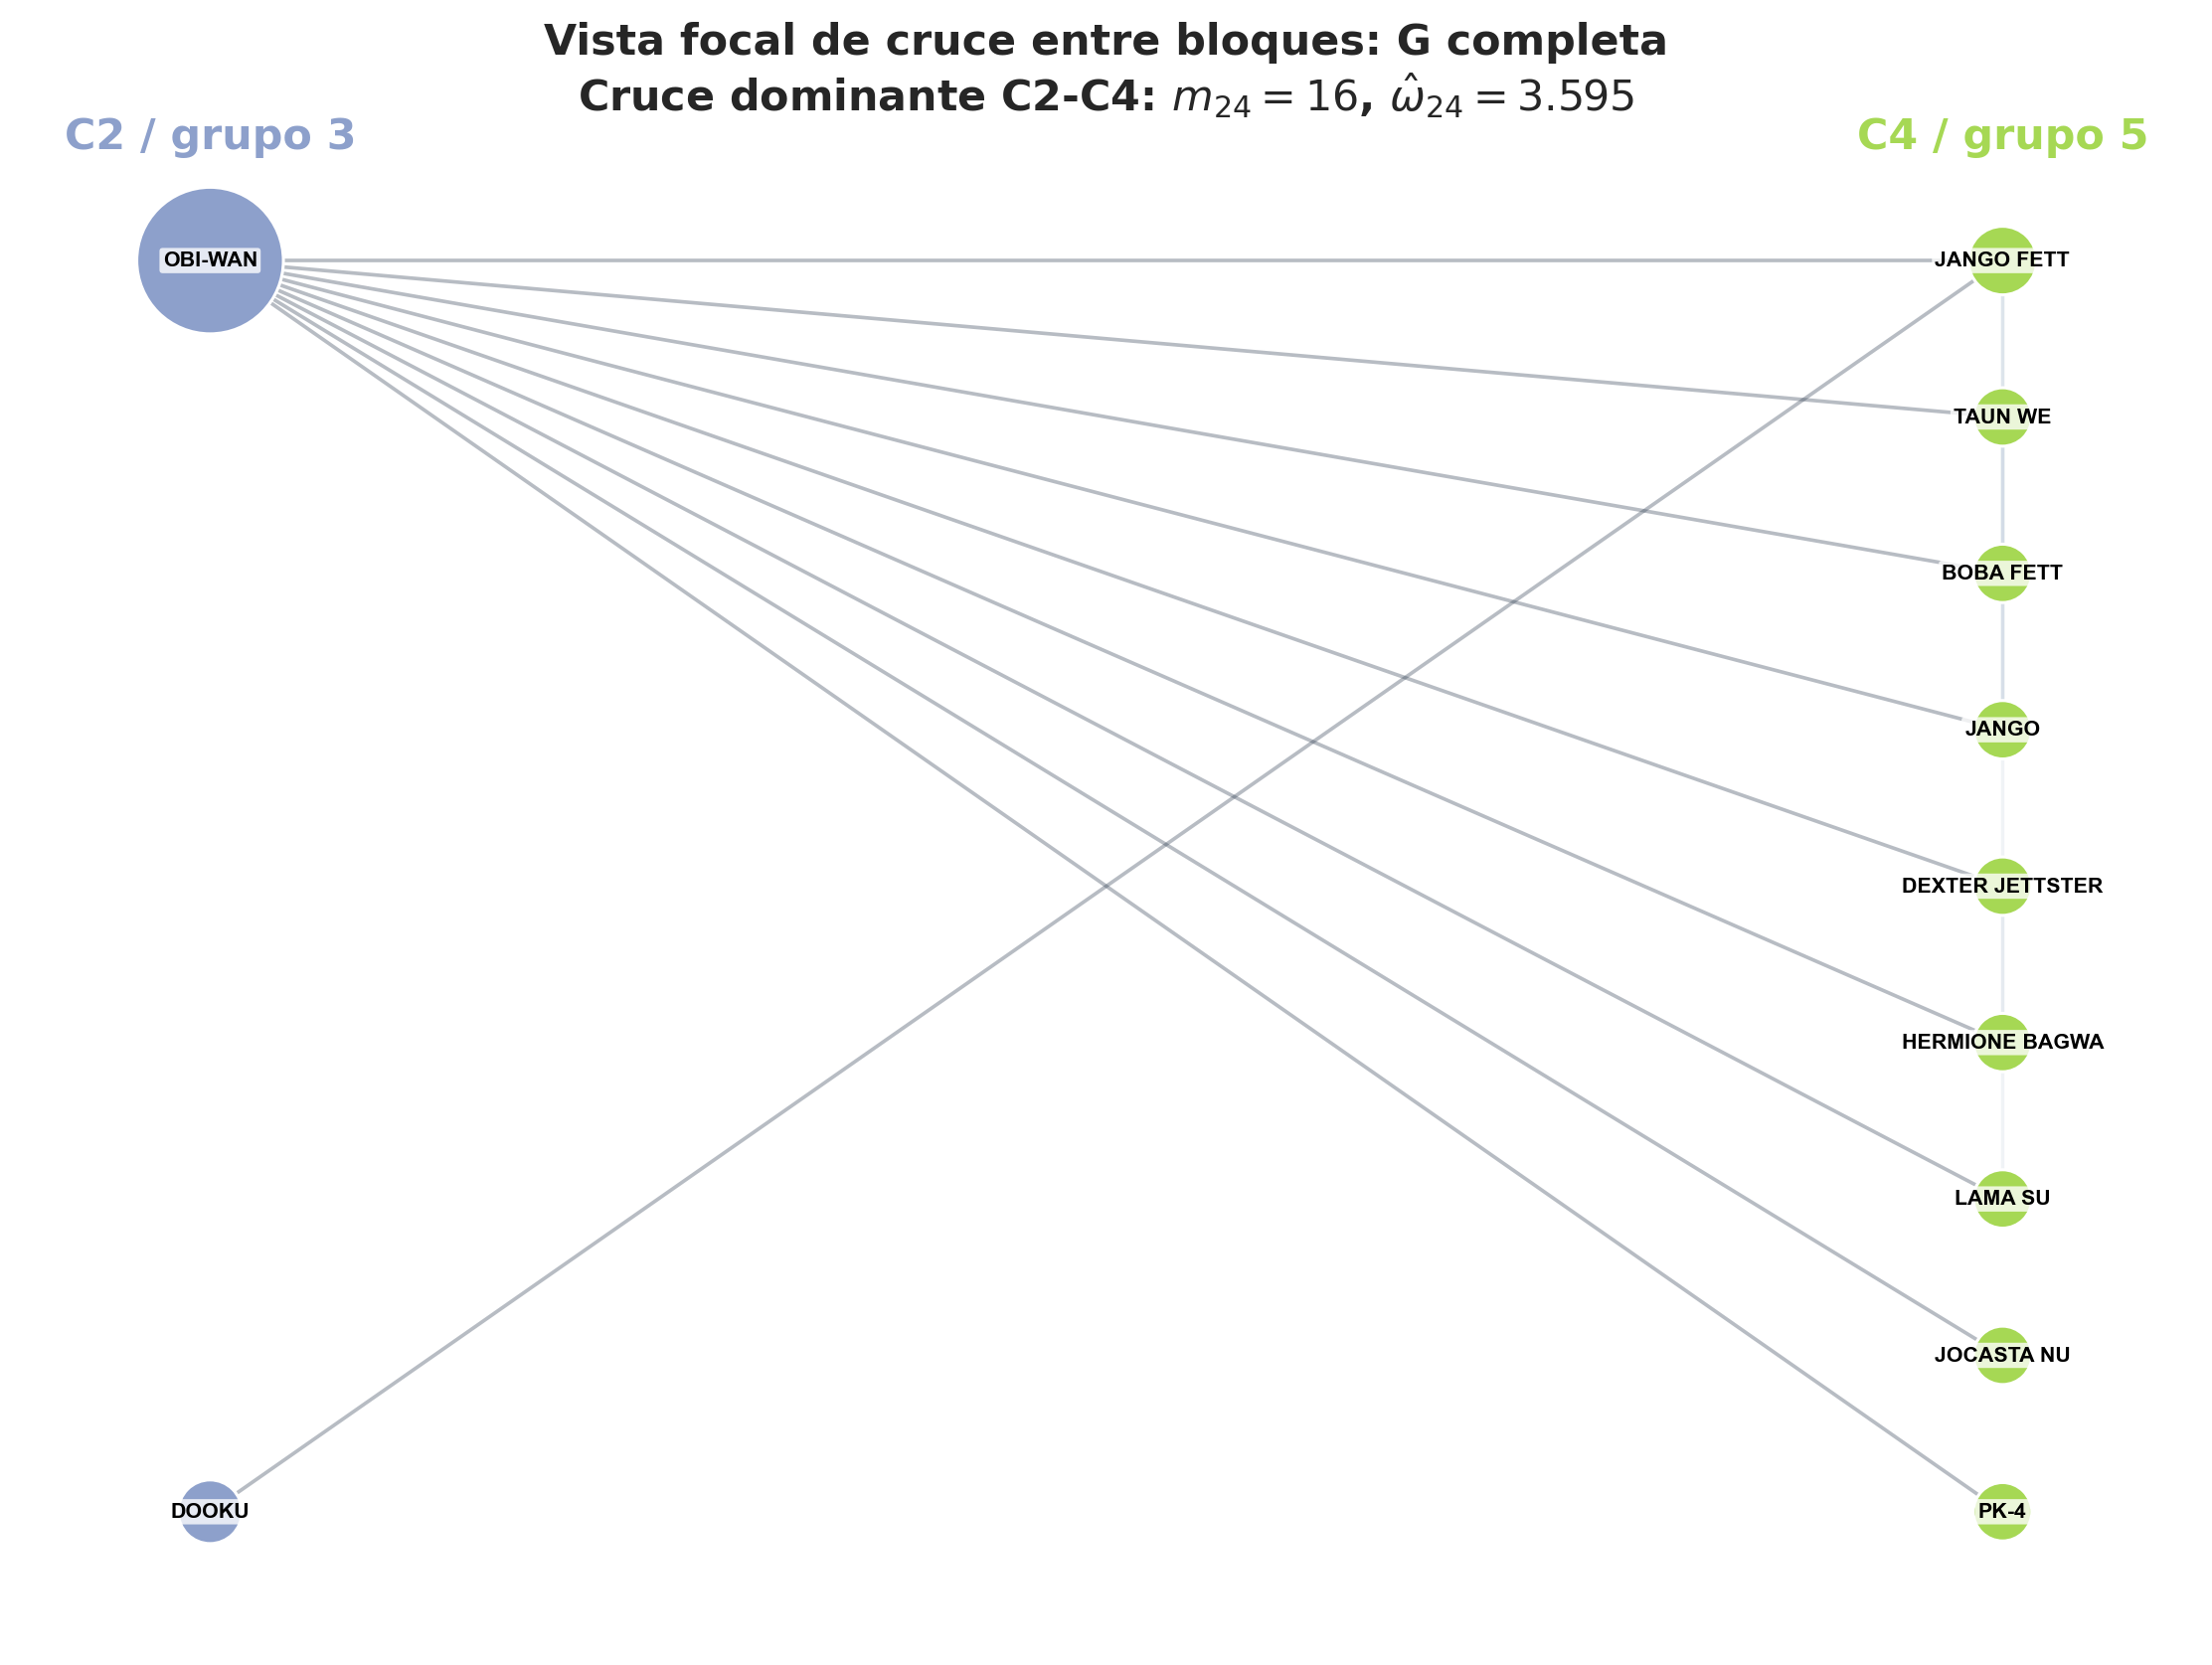
\includegraphics[height=0.55\textheight]{vista_cruce_dominante_G_completa.png}

\vspace{0.1cm}
\begin{block}{Interpretación específica}
\small
El cruce C2--C4, es decir grupos 3--5, tiene
\[
m_{35}=16,\qquad \what_{35}=3.595.
\]
Obi-Wan no queda simplemente dentro de Kamino/Jango: aparece como puente de investigación que conecta esa subtrama con el resto de la película.
\end{block}
\end{frame}

% ------------------------------------------------------------
\begin{frame}{Por qué Kamino/Jango tiene $\what_{55}=6.818$}
\begin{block}{Cálculo}
En la red completa:
\[
2m=296,\qquad m_{55}=18,\qquad \kappa_5=35.
\]
Entonces
\[
\what_{55}
=
\frac{296\cdot 18}{35^2}
=6.818.
\]
\end{block}

\begin{alertblock}{Interpretación}
No es solo que haya 18 unidades de masa interna. Es que esa masa es enorme para un bloque con volumen de grado $\kappa_5=35$. Por eso el modelo ve a Kamino/Jango como una subtrama muy concentrada.
\end{alertblock}
\end{frame}

% ------------------------------------------------------------
\begin{frame}{Por qué Senado/Jedi no tiene la $\omega$ más alta}
\begin{block}{Datos}
El grupo 6 tiene:
\[
m_{66}=110,\qquad \kappa_6=158.
\]
Entonces
\[
\what_{66}=2.045.
\]
\end{block}

\begin{alertblock}{Interpretación}
Aunque $m_{66}=110$ es enorme, el grupo 6 también tiene mucho volumen de grado. La corrección por grado reduce la sorpresa estadística: era esperable que un bloque con Yoda, Palpatine, Mace Windu, Jar Jar y senadores tuviera muchas conexiones.
\end{alertblock}
\end{frame}

% ------------------------------------------------------------
\begin{frame}{Red completa: adyacencia antes y después}
\centering
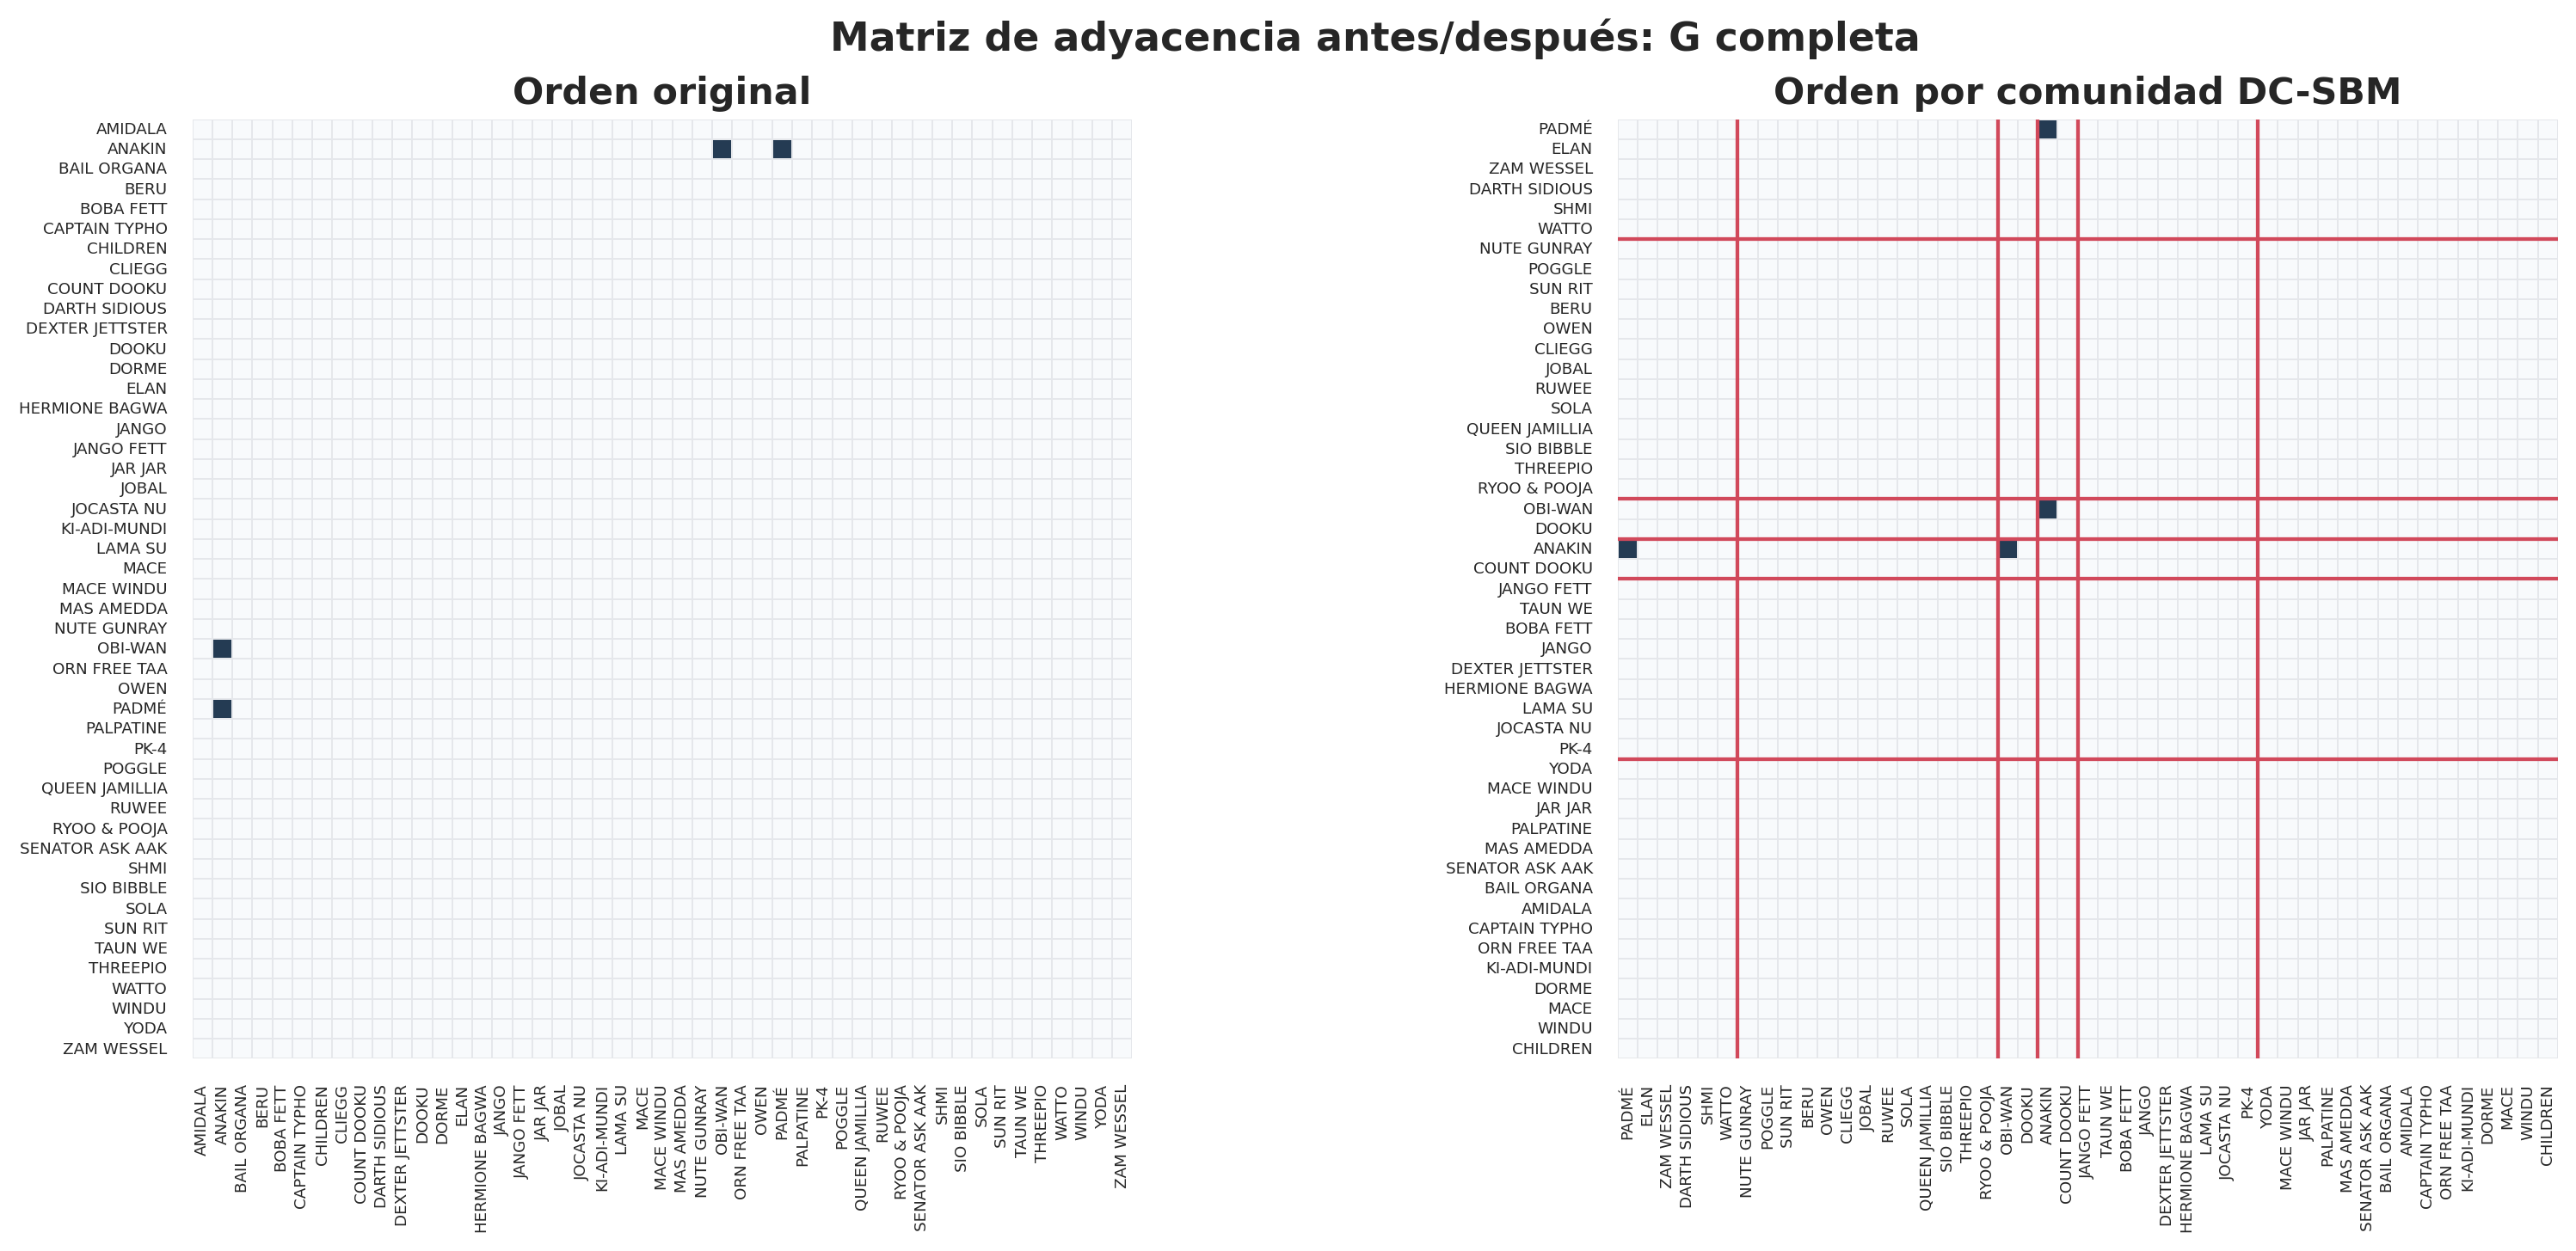
\includegraphics[height=0.60\textheight]{adyacencia_antes_despues_G_completa.png}

\vspace{0.1cm}
\begin{block}{Lectura}
\small
Ordenar por comunidad revela bloques diagonales y rectángulos fuera de la diagonal. La estructura se vuelve visible cuando los personajes se agrupan por el ajuste del DC-SBM.
\end{block}
\end{frame}

% ------------------------------------------------------------
\begin{frame}{Red completa: red partida}
\centering
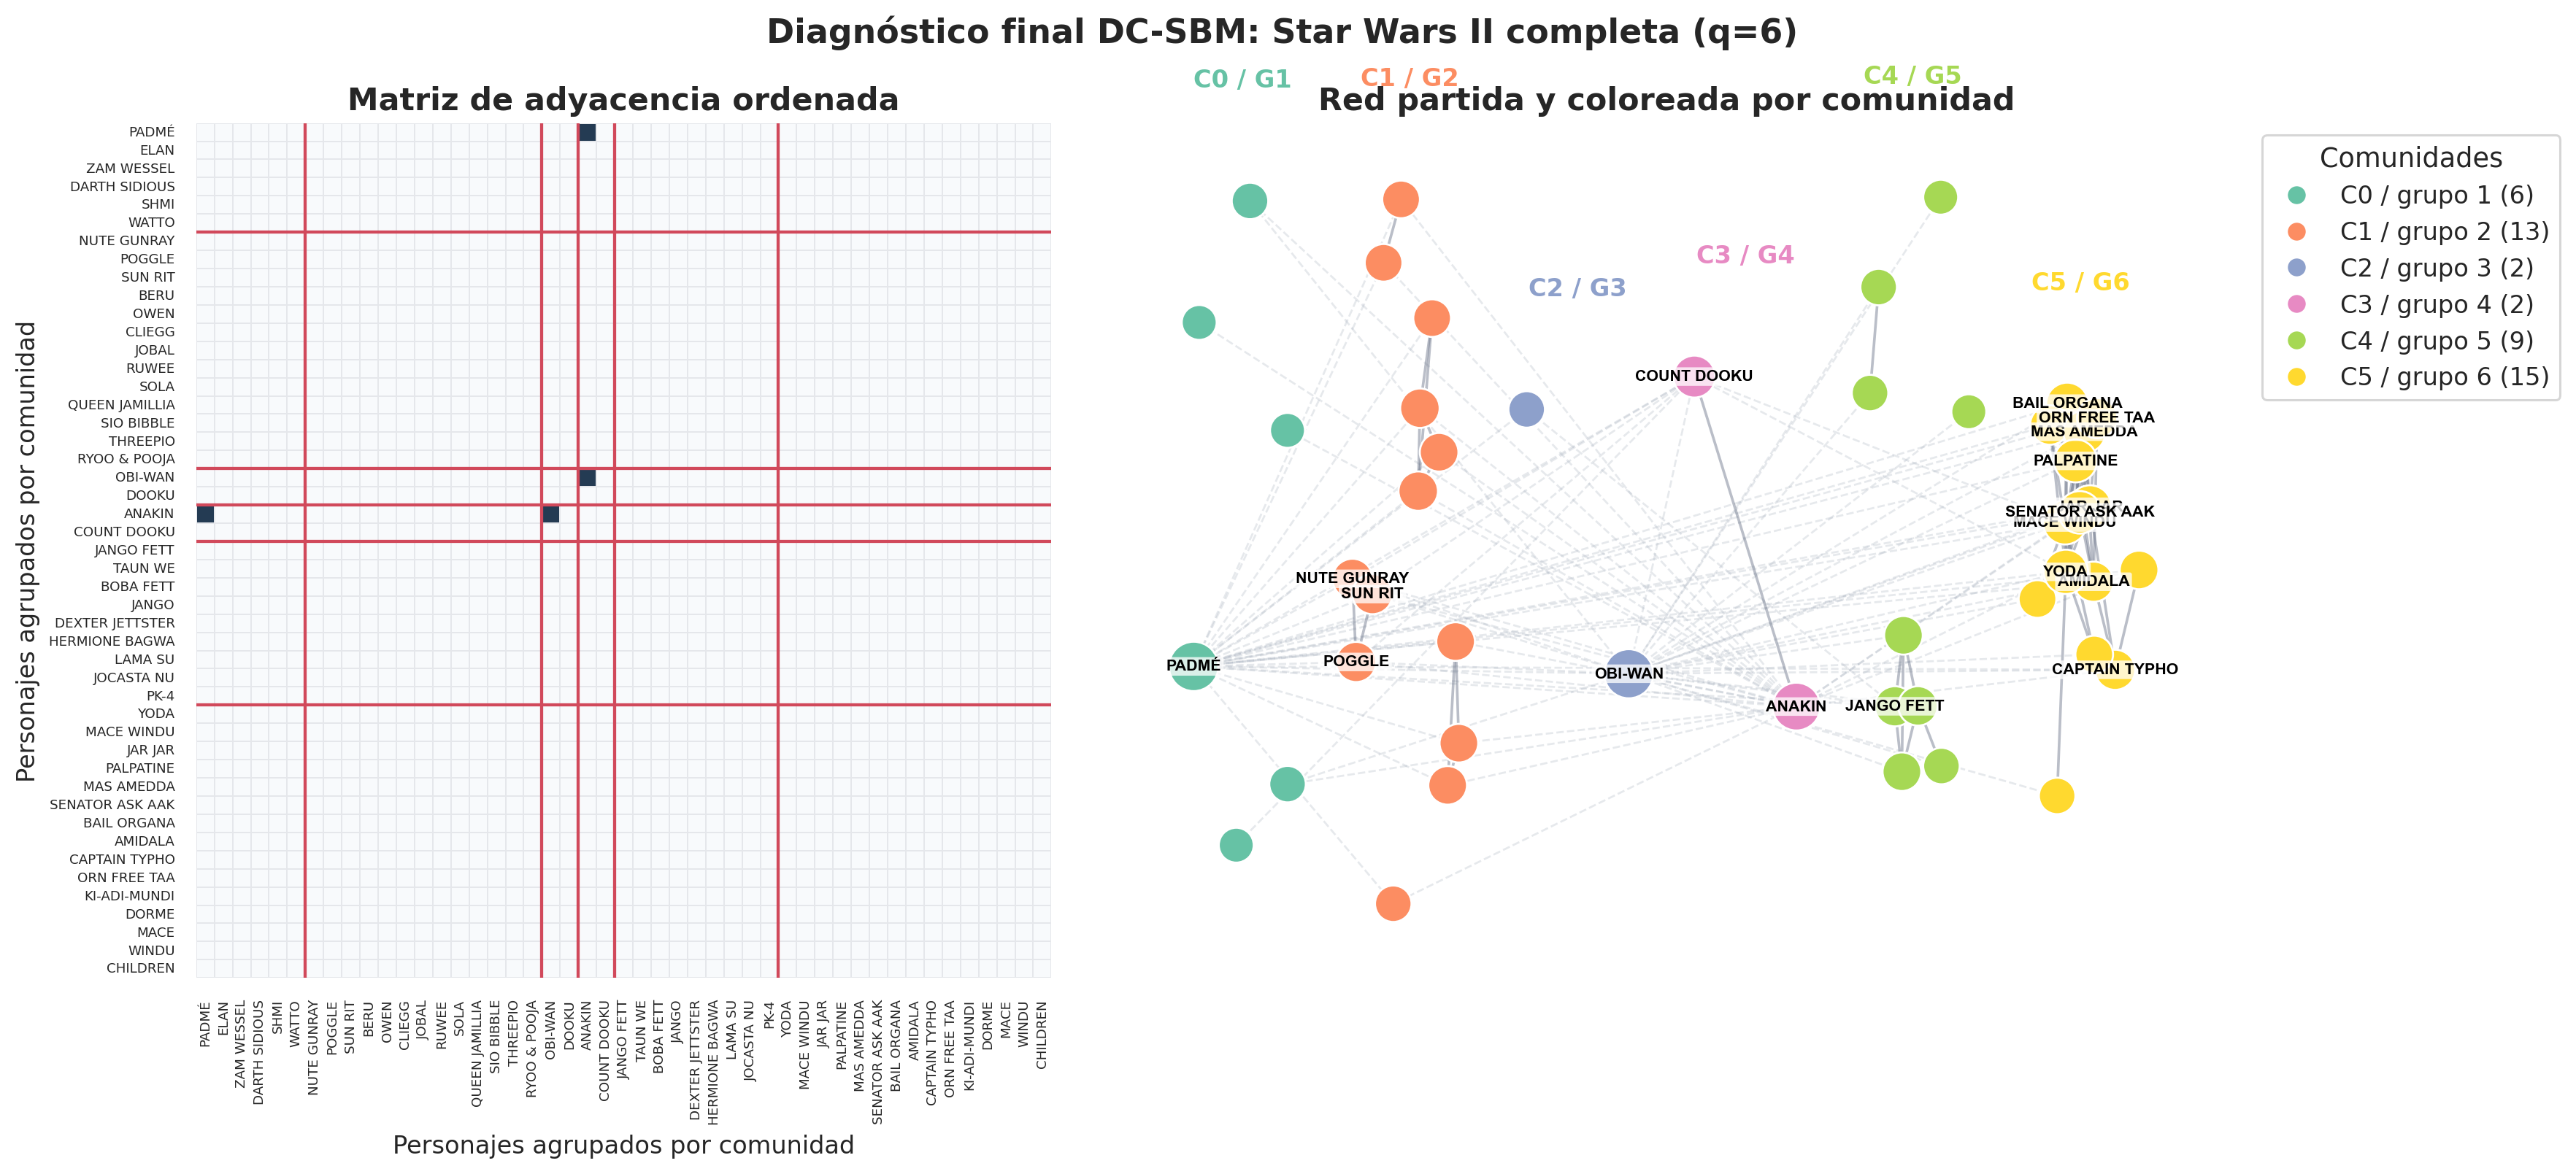
\includegraphics[height=0.78\textheight]{final_adyacencia_y_red_partida_G.png}
\end{frame}

% ------------------------------------------------------------
\section{Minired}

\begin{frame}{Minired: comunidades estimadas}
\scriptsize
\centering
\begin{tabular}{clrrp{7.2cm}}
\toprule
Grupo & Lectura & Nodos & Int. & Miembros\\
\midrule
1 & Puentes centrales & 2 & 1 & OBI-WAN, PADMÉ\\
2 & Tatooine/Naboo periférico & 13 & 12 & BERU, CLIEGG, DORME, NUTE GUNRAY, OWEN, POGGLE, THREEPIO\\
3 & Núcleo Kamino/Jango & 4 & 6 & BOBA FETT, JANGO, JANGO FETT, TAUN WE\\
4 & Senado/Jedi/República & 12 & 37 & AMIDALA, BAIL ORGANA, JAR JAR, MACE WINDU, PALPATINE, YODA\\
5 & Eje Anakin/Dooku/Typho & 3 & 2 & ANAKIN, CAPTAIN TYPHO, COUNT DOOKU\\
\bottomrule
\end{tabular}

\vspace{0.25cm}
\begin{block}{Lectura}
Al quitar personajes periféricos, la estructura se condensa: Obi-Wan y Padmé quedan como puentes centrales, y Kamino/Jango queda como núcleo cerrado.
\end{block}
\end{frame}

% ------------------------------------------------------------
\begin{frame}{Minired: dashboard}
\centering

\includegraphics[height=0.74\textheight]{dashboard_comunidades_G_mini.png}
\end{frame}

% ------------------------------------------------------------
\begin{frame}{Minired: matriz $M$}
\scriptsize
\[
M=
\begin{pmatrix}
8&23&8&31&37\\
23&34&0&0&18\\
8&0&14&0&0\\
31&0&0&102&11\\
37&18&0&11&4
\end{pmatrix}
\]

\begin{block}{Lectura}
\begin{itemize}
    \item $m_{33}=14$: el bloque Kamino/Jango es muy interno.
    \item $m_{44}=102$: Senado/Jedi conserva mucha masa interna.
    \item $m_{15}=37$: los puentes centrales conectan fuertemente con Anakin/Dooku/Typho.
\end{itemize}
\end{block}
\end{frame}

% ------------------------------------------------------------
\begin{frame}{Minired: matriz $\Omhat$}
\scriptsize
\[
\Omhat=
\begin{pmatrix}
0.292&1.198&1.421&0.841&2.065\\
1.198&2.527&0&0&1.433\\
1.421&0&12.091&0&0\\
0.841&0&0&2.056&0.456\\
2.065&1.433&0&0.456&0.341
\end{pmatrix}
\]

\begin{alertblock}{Lectura clave}
El núcleo Kamino/Jango tiene $\what_{33}=12.091$, una intensidad enorme. El cruce dominante fuera de diagonal es grupos 1--5, con $\what_{15}=2.065$.
\end{alertblock}
\end{frame}

% ------------------------------------------------------------
\begin{frame}{Radiografía de bloques: minired}
\centering

\includegraphics[width=0.96\textwidth]{radiografia_bloques_G_mini.png}
\end{frame}

% ------------------------------------------------------------
\begin{frame}{Cruce dominante de la minired}
\centering
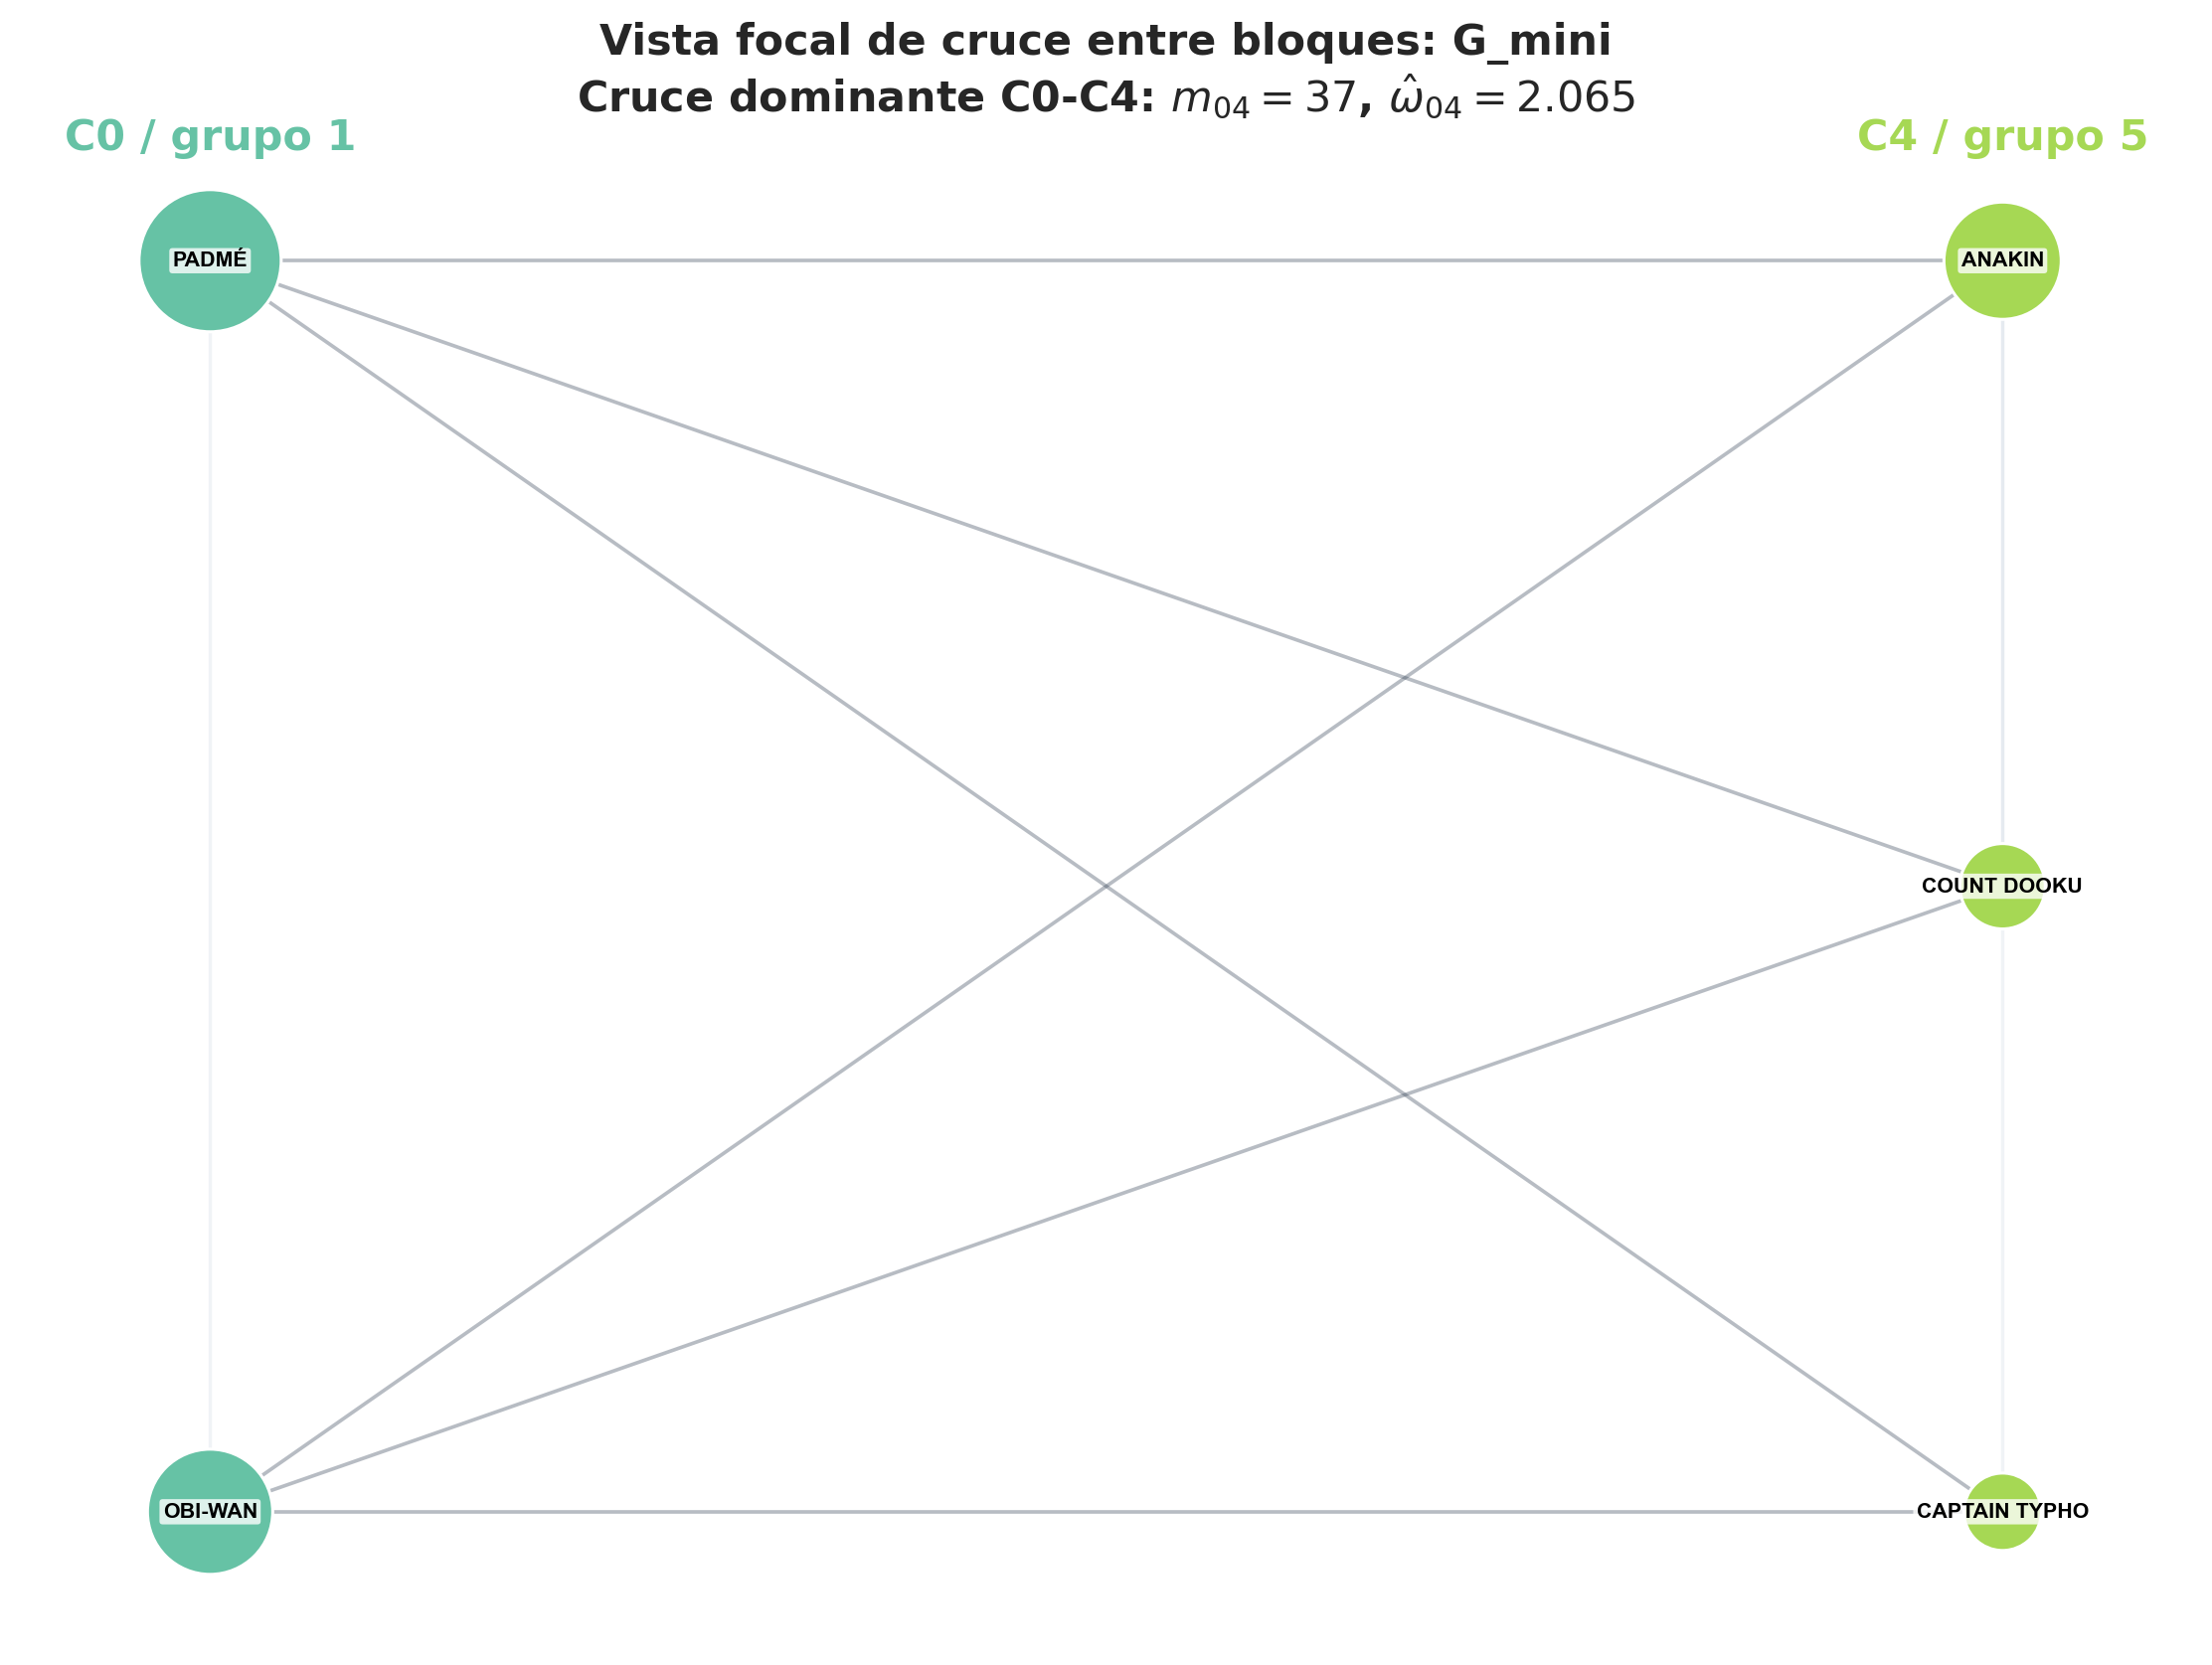
\includegraphics[height=0.55\textheight]{vista_cruce_dominante_G_mini.png}

\vspace{0.1cm}
\begin{block}{Interpretación específica}
\small
El cruce grupos 1--5 tiene
\[
m_{15}=37,\qquad \what_{15}=2.065.
\]
Padmé y Obi-Wan conectan con Anakin, Count Dooku y Captain Typho: la red central mezcla romance, investigación y conflicto político.
\end{block}
\end{frame}

% ------------------------------------------------------------
\begin{frame}{Por qué Kamino/Jango se vuelve más claro en la minired}
\begin{block}{Cálculo}
En la minired:
\[
2m=256,\qquad m_{33}=14,\qquad \kappa_3=22.
\]
Entonces
\[
\what_{33}
=
\frac{256\cdot 14}{22^2}
=12.091.
\]
\end{block}

\begin{alertblock}{Interpretación}
Al retirar nodos periféricos, queda un grupo pequeño pero casi cerrado. La intensidad corregida crece mucho porque la masa interna es grande comparada con el volumen del bloque.
\end{alertblock}
\end{frame}

% ------------------------------------------------------------
\begin{frame}{Minired: adyacencia ordenada y red partida}
\centering

\includegraphics[width=0.92\textwidth]{final_adyacencia_y_red_partida_G_mini.png}
\end{frame}

% ------------------------------------------------------------
\section{Síntesis}

\begin{frame}{Comparación: red completa vs minired}
\centering
\small
\begin{tabular}{lll}
\toprule
Elemento & Red completa & Minired\\
\midrule
$q$ seleccionado & 6 & 5\\
Bloque más intenso & Kamino/Jango & Kamino/Jango\\
Mayor $\omega$ & $\what_{55}=6.818$ & $\what_{33}=12.091$\\
Cruce dominante & Obi-Wan--Kamino/Jango & Puentes--Anakin/Dooku/Typho\\
Lectura global & subtramas + roles & núcleo narrativo condensado\\
\bottomrule
\end{tabular}

\vspace{0.35cm}
\begin{block}{Qué se conserva}
En ambas redes aparece una subtrama Kamino/Jango muy compacta y un bloque Senado/Jedi/República. La minired hace más visible el papel de los protagonistas como puentes.
\end{block}
\end{frame}

% ------------------------------------------------------------
\begin{frame}{Qué aprendimos del método}
\begin{enumerate}
    \item La corrección por grado evita confundir protagonistas con comunidades.
    \item $M$ muestra dónde están las aristas observadas.
    \item $\Omhat$ muestra qué conexiones son fuertes después de corregir por grado.
    \item Diagonales grandes indican subtramas densas.
    \item Fuera de diagonal grande indica relación entre roles narrativos.
\end{enumerate}

\vspace{0.25cm}
\begin{alertblock}{Mensaje metodológico}
El DC-SBM es útil cuando la red no es puramente modular. En historias, organizaciones y mercados, los roles pueden ser tan importantes como las comunidades.
\end{alertblock}
\end{frame}

% ------------------------------------------------------------
\begin{frame}{Interpretación específica de la película}
\begin{itemize}
    \item \textbf{Kamino/Jango} aparece como subtrama cerrada: Jango, Boba, Taun We, Lama Su y personajes asociados.
    \item \textbf{Senado/Jedi/República} aparece como bloque grande y denso, pero menos sorprendente después de corregir por grado.
    \item \textbf{Obi-Wan} funciona como puente de investigación hacia Kamino/Jango.
    \item \textbf{Padmé y Anakin} conectan la parte emocional/política con el conflicto central.
    \item \textbf{La minired} revela con más claridad los roles de protagonistas puente.
\end{itemize}
\end{frame}

% ------------------------------------------------------------
\begin{frame}{Conclusión final}
\centering
\Large
\[
\boxed{
\text{subtramas densas}
\quad+\quad
\text{protagonistas puente}
\quad+\quad
\text{cruces entre roles narrativos}
}
\]

\vspace{0.5cm}
\normalsize
El DC-SBM muestra que la red de \emph{Attack of the Clones} no se reduce a comunidades aisladas. La película está organizada por subtramas, pero los protagonistas conectan esas subtramas de manera estadísticamente visible.
\end{frame}

% ------------------------------------------------------------
\begin{frame}{Archivos generados}
\begin{itemize}
    \item Notebook: \texttt{02 Star Wars.ipynb}
    \item Resultados: \texttt{outputs\_sbm\_sw/}
    \item Reporte: \texttt{resultados\_star\_wars\_dc\_sbm.tex}
    \item Presentación: \texttt{presentacion\_star\_wars\_dc\_sbm.tex}
\end{itemize}

\vspace{0.3cm}
\begin{block}{Reproducibilidad}
La notebook ejecuta el ajuste, exporta tablas CSV, guarda las figuras y deja los resultados listos para el reporte y la presentación.
\end{block}
\end{frame}

\end{document}
